\documentclass[crop,tikz]{standalone} 
\usepackage{tikz, amsmath, amssymb, graphicx} 

\DeclareMathAlphabet\mathbfcal{OMS}{cmsy}{b}{n}

\newcommand{\Mt}{\mathbfcal{M}}
\newcommand{\Yt}{\mathbfcal{Y}}
\newcommand{\Ft}{\mathbfcal{F}}

\usetikzlibrary{positioning, shapes.geometric} 

\begin{document}  

\tikzset{fontscale/.style = {font=\relsize{#1}}
    }

\begin{tikzpicture} 

 
\node[inner sep=0pt] at (0, 0) {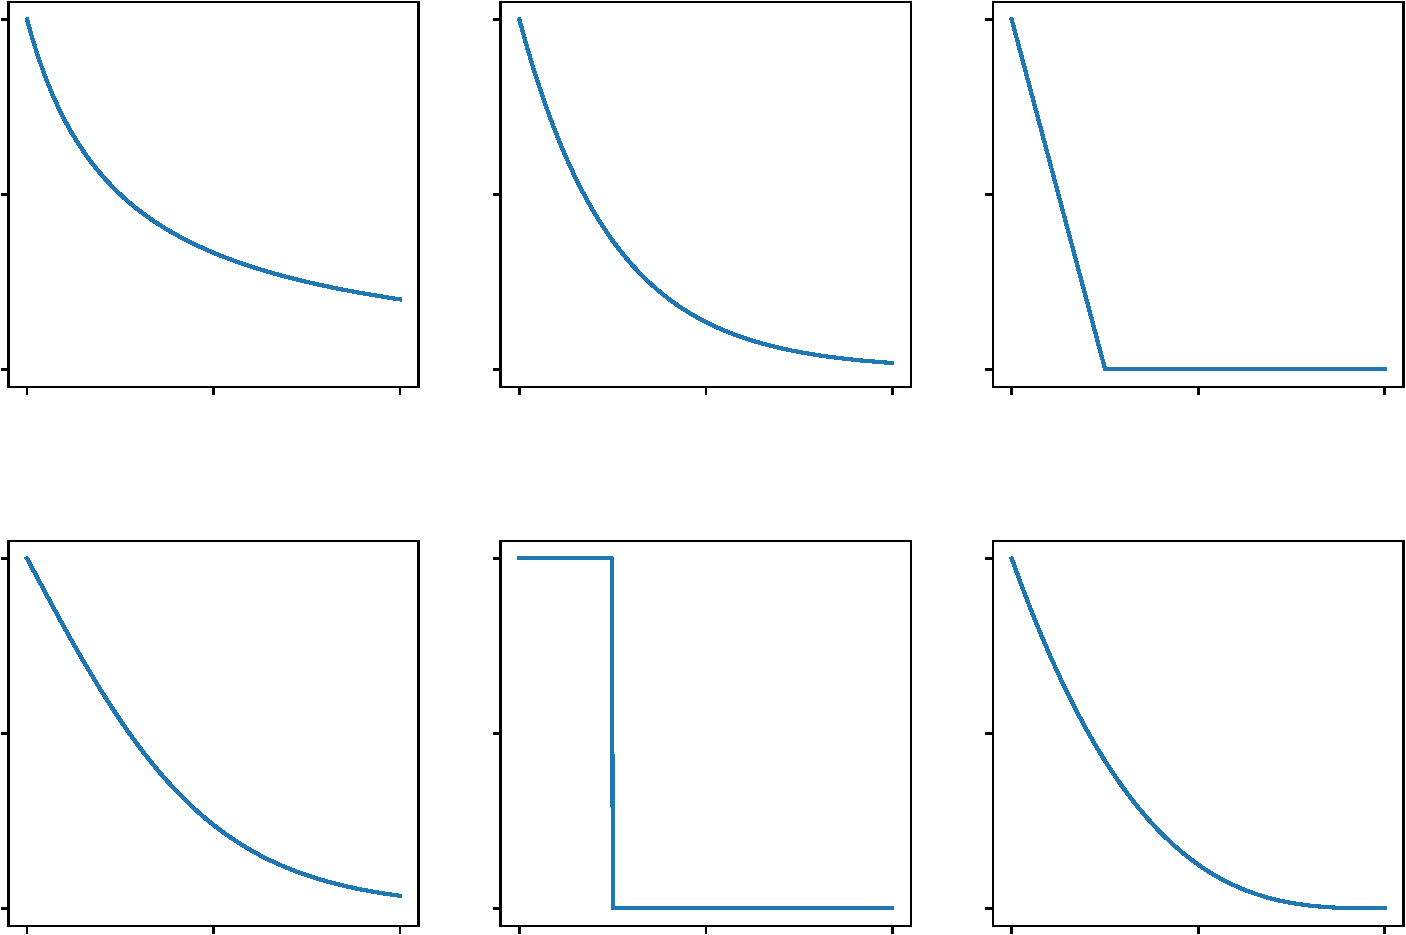
\includegraphics[width=.22\textwidth]{filters.pdf}};
\node[inner sep=0pt, scale=0.3] at (-0.93, 0.97) {One-hop};
\node[inner sep=0pt, scale=0.3] at (0, 0.97) {Diffusion};
\node[inner sep=0pt, scale=0.3] at (0.93, 0.97) {RuLu};
\node[inner sep=0pt, scale=0.3] at (-0.93, -0.05) {Sigmoid};
\node[inner sep=0pt, scale=0.3] at (0, -0.05) {Bandlimited};
\node[inner sep=0pt, scale=0.3] at (0.93, -0.05) {Polynomial};


\node[inner sep=0pt, scale=0.25] at (-1.28, -0.97) {$0$};
\node[inner sep=0pt, scale=0.25] at (-0.35, -0.97) {$0$};
\node[inner sep=0pt, scale=0.25] at (0.59, -0.97) {$0$};

\node[inner sep=0pt, scale=0.25] at (-0.55, -0.97) {$\lambda_{\text{max}}$};
\node[inner sep=0pt, scale=0.25] at (0.37, -0.97) {$\lambda_{\text{max}}$};
\node[inner sep=0pt, scale=0.25] at (1.32, -0.97) {$\lambda_{\text{max}}$};


\node[inner sep=0pt, scale=0.25] at (-1.4, -0.84) {$0$};
\node[inner sep=0pt, scale=0.25] at (-1.43, -0.51) {$0.5$};
\node[inner sep=0pt, scale=0.25] at (-1.4, -0.17) {$1$};


\node[inner sep=0pt, scale=0.25] at (-1.4, 0.18) {$0$};
\node[inner sep=0pt, scale=0.25] at (-1.43, 0.51) {$0.5$};
\node[inner sep=0pt, scale=0.25] at (-1.4, 0.85) {$1$};

\end{tikzpicture}
\end{document} 
